\begin{section}{Desarrollo}
	\begin{subsection}{Explicación}
		Para construir la curva parámetrica se puede utilizar cualquiera de las $tres$ parametrizaciones (uniforme, chord-length y centrípeta) en el intervalo $[0,1]$.
		La parametrización $t$ se elige a partir de los puntos de control $(x,y)$ recibidos en la entrada del programa.
		Una vez elegida la parametrización se generan dos splines, el primero $S_x$ a partir del par $(t,x)$ y el otro $S_y$ a partir de $(t,y)$.
		De esta manera, queda definida una curva $C \in \mathbb{R}^2$ donde $C(t) = (S_x(t),S_y(t))$.
		
		Para mover un punto $(x,y)$ cercano a la curva a una nueva posición $(x*,y*)$, calculamos primero el punto de la curva más próximo a $(x,y)$ y luego construimos una nueva curva (manteniendo la parametrización original) de manera tal que ambas splines ($S_x$ y $S_y$) ahora pasen también por la nueva posición $(x*,y*)$.
		
		Para calcular el punto de la curva más próximo a $(x,y)$ minimizamos (derivamos y buscamos donde se anula distinguiendo entre máximos y mínimos) la	función distancia$^1$ de la curva al punto $(x,y)$ en cada intervalo $[t_i,t_{i+1}] \in [0,1]$ (polinomio que la conforma) y luego seleccionamos el mínimo en $[0,1]$.\\
		
		A continuación se detalla la busqueda del punto más cercano a la curva dado $(x,y)$.
		
		Sea $n$ la cantidad de puntos de control y $S_x^i$, $S_y^i$ el $i-esimo$ polinomio de cada spline de la curva.\\
		 
		$t /\; min\; \sqrt{(S_x(t)-x)^2+(S_y(t)-y)^2} \left\{
		\begin{array}{c}
		t_1 /\; min\; \sqrt{(S_x^{(1)}(t)-x)^2+(S_y^{(1)}(t)-y)^2}\\
		t_2 /\; min\; \sqrt{(S_x^{(2)}(t)-x)^2+(S_y^{(2)}(t)-y)^2}\\
		\vdots\\
		t_{n-1} /\; min\; \sqrt{(S_x^{(n-1)}(t)-x)^2+(S_y^{(n-1)}(t)-y)^2}\\
		\end{array}
		\right.$
		\VSP		
	\end{subsection}
	\begin{subsection}{Implementación}
		La implementación esta divida en módulos que realizan tareas específicas, a continuación detallaremos cada uno de ellos.
		
		\begin{itemize}
			\item \underline{Módulo Parametrización:}\\
				Este módulo implementa las $tres$ parametrizaciones (uniforme,\\
				chord-length, centrípeta) en el $[0,1]$ dado un conjunto de puntos de control.
		
			\item \underline{Módulo Spline:}\\
				Escribimos el módulo \texttt{Spline} que implementa un spline cúbico natural con las siguientes operaciones:\\
				
				\begin{tabular}{rl}
					\texttt{Evaluar} & Evalua la spline (buscando previamente el polinomio \\
									 & correspondiente) en un valor recibido como parámetro.\\
					\texttt{Polinomio} & Devuelve el polinomio requerido.\\
				\end{tabular}\\

			\item \underline{Módulo Curva:}\\
				El módulo \texttt{Curva} implementa una curva parámetrica con las siguientes operaciones:\\
				
				\begin{tabular}{rl}
					\texttt{Punto cercano} & Dadas las coordenadas de un punto cercano a la curva, calcula\\
										   & el punto de la curva más próximo.\\
					\texttt{Mover punto} & Dadas las coordenadas de un punto cercano a la curva, calcula el\\
										 & punto de la curva más próximo y construye una nueva spline\\
										 & resultante de modificar la spline original de manera que ahora\\
										 & pase por la nueva posición del punto seleccionado.\\
					\texttt{Muestreo} & Devuelve un muestreo de la curva.\\
				\end{tabular}\\
				
				Esta clase cuenta con un método $private$ (que se usa tanto para \texttt{'Punto cercano'} como para \texttt{'Mover Punto'}) que busca el $t \in [0,1]$ tal que al evaluar la curva en $t$ se obtiene el punto más cercano a la misma respecto de un punto dado $(x,y)$.
				
				Se busca el $t$ que minimiza la función distancia\footnote{Distancia euclídea de $(S_x(t),S_y(t))$ a $(x,y)$: $\sqrt{(S_x(t)-x)^2+(S_y(t)-y)^2}$} del punto $(x,y)$ a cada polinomio de la curva en el intervalo correspondiente ($[t_i,t_{i+1}]$) y se verifica si se puede actualizar el mínimo global, es decir, se selecciona el $t$ que minimiza la distancia en $[t_1,t_{i+1}]$.
				
				Llamamos $d_i(t)$ a la distancia de $(S_x^{(i)}(t),S_y^{(i)}(t))$ a $(x,y)$, es decir, la distancia a la curva en el intervalo $[t_i,t_{i+1}]$ ($i-esimo$ polinomio).\\
				
				Como la función distancia ($d_i(t)$) es monótona creciente en $\mathbb{R}_{>0}$ podemos minimizar $d_i^2(t)$ ya que coinciden en los puntos críticos (mínimo y máximo).\\
				
				$d_i^2(t) = (S_x^{(i)}-x)^2+(S_y^{(i)}-y)^2$\\
				
				Sea $z=(t-t_i) \Rightarrow$
				
				$d_i^2(t) = (a_{x_i} + b_{x_i}*z + c_{x_i}*z^2 + d_{x_i}*z^3 - x)^2 + (a_{y_i} + b_{y_i}*z + c_{y_i}*z^2 + d_{y_i}*z^3 -y)^2$\\
				
				Para minimizar $d_i^2(t)$ obtenemos la derivada:.
				
				$(d_i^2)'(t) = 2(S_x^{(i)}(t)-x)(S_x^{(i)}(t)-x)'+2(S_y^{(i)}(t)-y)(S_y^{(i)}(t)-y)'$\\
				
				Sea $E_{k_i} = 2(S_k^{(i)}(t)-k)(S_k^{(i)}(t)-k)'$ \\
				
				$E_{k_i} = 2b_{k_i}(a_{k_i}-k)+2(b_{k_i}^2+2c_{k_i}(a_{k_i}-k))*z+6(c_{k_i}b_{k_i}+d_{k_i}(a_{k_i}-k)))*z^2+4(2d_{k_i}b_{k_i}+c_{k_i}^2)*z^3+10d_{k_i}c_{k_i}*z^4+6d_{k_i}^2*z^5$\\
				
				$\Rightarrow (d_i^2)'(t) = E_{x_i} + E_{y_i}$\\
				
				\underline{\texttt{Nota:}} Esta expresión se encuentra 'hardcodeada' en una función $private$ que devuelve el polinomio 'distancia' derivado a partir de los coeficientes de $S_x$, $S_y$.
				
				Por último, buscamos los $t$ donde $(d_i^2)'(t)$ se anula. Estos $t$ que son los puntos críticos de la función corresponden a máximos o a mínimos.
				Nos quedamos con el $t$ tal minimiza $d(t)$.
				
				A continuación exponemos el pseudocódigo de esta función con el objetivo de esclarecer su explicación:\\
				
				\begin{pseudo}
					\func{PuntoMásProx}{$curva$,$(x,y)$}\\
					\tab $min\_global = 0$\\
					\tab \FOR $i\gets 1 \TO cantPtosControl-1$\\
					\tab\tab $pol_i = distDerivada(curva,(x,y),i)$\\
					\tab\tab $ptosCriticos = ceros(pol_i,i,i+1)$\\
					\tab\tab $min\_t = minimo(ptosCriticos)$\\
					\tab\tab $dist\_min\_global = dist(S_x(min\_global),S_y(min\_global),x,y)$\\
					\tab\tab $dist\_min\_t = dist(S_x(min\_t),S_y(min\_t),x,y)$\\
					\tab\tab \IF $dist\_min\_t < dist\_min\_global$ \THEN\\
					\tab\tab\tab $dist\_min\_global = dist\_min_t$\\
					\tab \RET $(S_x(min\_global),S_y(min\_global))$\\
				\end{pseudo}
				
				Para mover un punto $(x,y)$	calculamos el punto de la curva más próximo como se explicó previamente. Luego, separamos en los siguientes casos:
				
				\begin{itemize}
					\item \underline{Caso punto más cercano a $(x,y)$ es un punto de control:}\\
					
						Se reemplaza el punto de control (aquel que es el punto más próximo a $(x,y)$) por la posición final de $(x,y)$ y se construye una nueva curva a partir de los nuevos puntos de control manteniendo la parametrización.\\
						
						La siguiente figura ejemplifica este caso.\\
						
						\begin{figure}[H]
							\centering
							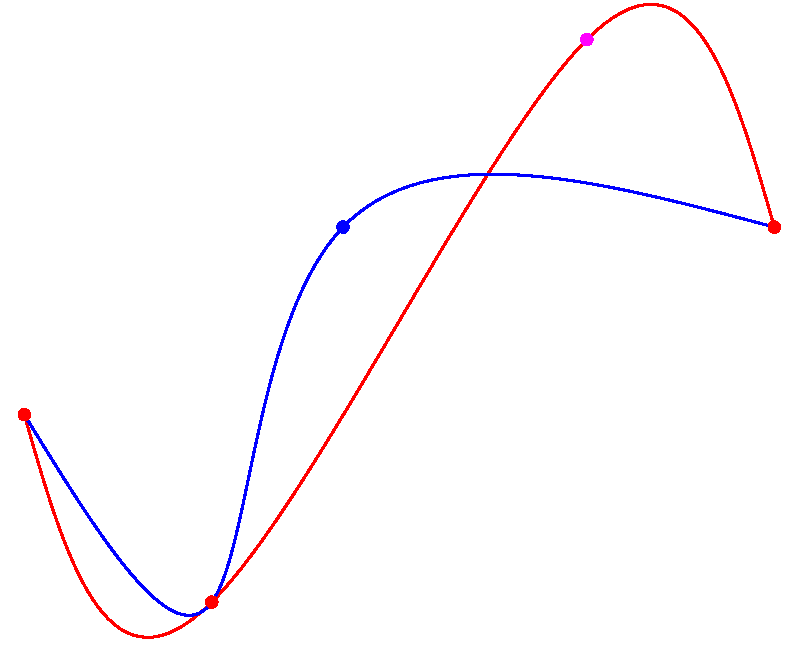
\includegraphics[width=7cm]{graficos/ptoCtrl.pdf}
							\caption{Punto más próximo a la curva corresponde a un punto de control de la misma}
							\label{fig:ptoCtrl}
						\end{figure}
						
						\VSP
						
						En este caso, la curva original ($roja$) se construyó a partir de $cuatro$ puntos de control (los puntos $rojos$ y el $rosa$), se seleccionó el punto $rosa$ por lo que sí mismo es el más cercano y se lo desplazó
						como ya se explicó a la posición donde está el punto $azul$.
						
						\VSP 
					
					\item \underline{Caso punto más cercano a $(x,y)$ no es un punto de control:}\\
					
						Se agrega como nuevo punto de control $(x*,y*)$ (posición final de $(x,y)$), además se agrega el $t$ correspondiente a la parametrización (la paramerización para el resto de los puntos de control se mantiene).
						Para esto, se selecciona la posición que le corresponde a estos datos según un orden creciente de $t$. Luego, se construye una nueva curva que ahora también pase por $(x*,y*)$.\\
						
						La siguiente figura es un ejemplo de esto, donde el punto seleccionado no está sobre la curva y el punto más próximo a este no es un punto de control.\\
						
						\begin{figure}[H]
							\centering
							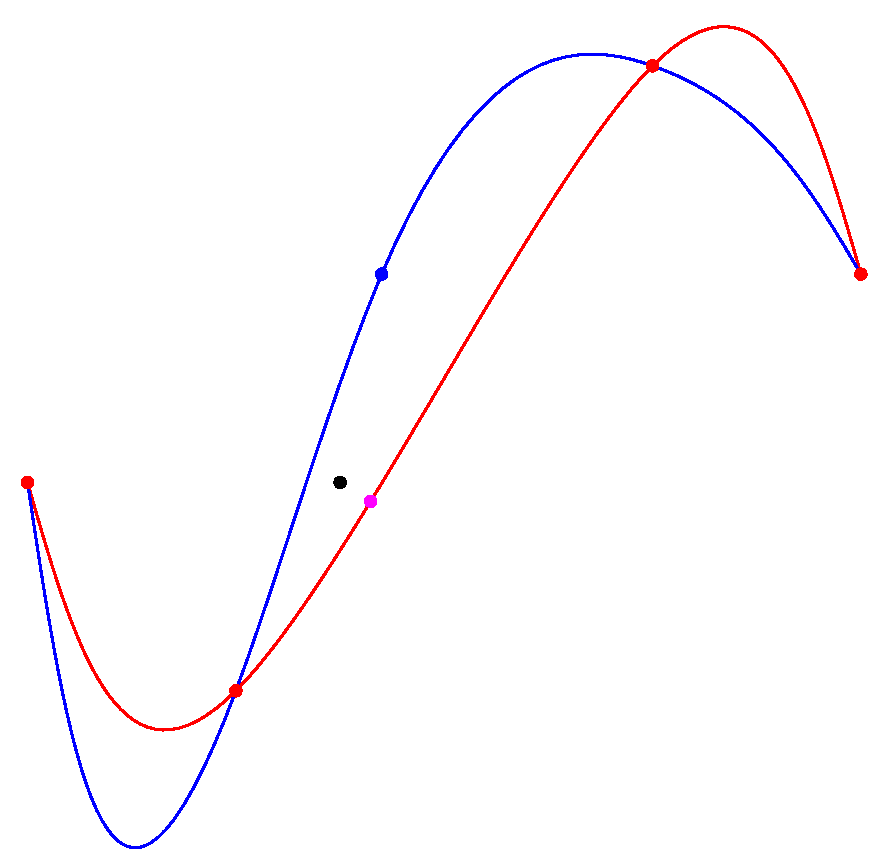
\includegraphics[width=6cm]{graficos/noPtoCtrl_noSobreCurva.pdf}
							\caption{El punto seleccionado no pertenece a la curva y el punto más próximo no es un punto de control}
							\label{fig:noPtoCtrl_noSobreCurva}
						\end{figure}
						
						\VSP
						
						La curva $roja$ corresponde a la curva original y los puntos $rojos$ a los puntos de control provistos para su construcción.
						
						El punto $negro$ es el punto seleccionado para ser movido, y el $rosa$ el punto perteneciente a la curva más próximo a este.
						
						La curva $azul$ es la curva deformada de forma tal que el punto $rosa$ toma la posición del punto $azul$.\\
						
						Por último, la siguiente figura refleja el comportamiento cuando el punto seleccionado está sobre la curva.\\
						
						\begin{figure}[H]
							\centering
							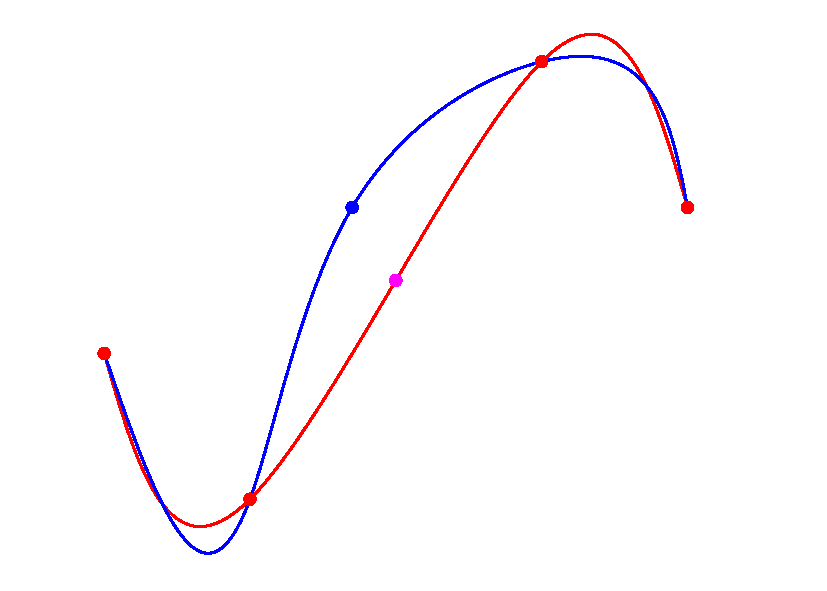
\includegraphics[width=9cm]{graficos/sobreCurva.pdf}
							\caption{Punto seleccionado pertenece a la curva pero no es un punto de control}
							\label{fig:sobreCurva}
						\end{figure}
				\end{itemize}
				
				\VSP
				
				Como en las figuras anteriores la curva $roja$ corresponde a la curva original. Los puntos de control son lo de color
				$rojo$. 
				
				El punto seleccionado se ve en color $rosa$ porque el punto perteneciente a la curva más próximo es sí mismo. Finalmente, vemos en $azul$ la curva
				deformada y la posición final del punto elegido.
				
				\VSP
				
				La última de las operaciones de la clase $curva$ (muestreo) selecciona $m$ puntos de muestreo, donde $m$ es recibido en la entrada.
				Estos puntos corresponden a un muestreo uniforme del rango del parámetro $([0,1])$ incluyendo los extremos.\\
				
				\item \underline{Módulo Polinomio:}\\
				Escribimos el módulo \texttt{Polinomio} que implementa un polinomio de\\
				grado $n$ con las siguientes operaciones:\\
				
				\begin{tabular}{rl}
					\texttt{Evaluar} & Evalua el polinomio en un valor recibido por parámetro.\\
					\texttt{Derivar} & Realiza la derivada primera del polinomio.\\
					\texttt{Ceros}   & Busca una raíz del polinomio usando bisección y el método\\
									 & de Newton.\\
				\end{tabular}\\ 
				
				Para encontrar los ceros de un polinomio en el intervalo $[a,b]$ implementamos un algortimo heurístico que detallamos a continuación:\\
				
				\begin{pseudo}
					\func{ceros}{$polinomio$,$a$,$b$}\\
					\tab $long\_intervalo = (b-a)/grado(polinomio)$\\
					\tab $b = a+long\_intervalo$\\
					\tab \FOR $i\gets 0 \TO grado(polinomio)-1$\\
					\tab\tab\tab $raices[i] = BuscarRaiz(polinomio,a,b)$\\
					\tab\tab\tab $a = b$\\
					\tab\tab\tab $b = b + long\_intervalo$\\
					\tab \RET $raices$\\
				\end{pseudo}
		
				Dado que el polinomio tiene a lo sumo tantas raíces como su grado, dividimos $[a,b]$ en esa cantidad de intervalos, apostando a que
				las mismas se encuentran uniformemente distribuídas, si esto sucede encontramos una raíz en cada intervalo. Para buscar cada una de 
				ellas ejecutamos el método de bisección mientras sea posible (cambie de signo en el intervalo) o hasta acercarnos lo suficiente
				(parámetro definido por nosotros, ver subsección 'Ajuste de parámetros' en la sección de resultados así como discusión). En ambos casos el algoritmo aplica en última instancia el método de $Newton$.\\
				En los intervalos donde no hay ninguna raíz el procedimiento es el mismo, el valor conseguido es producto de que el método de 
				$Newton$ utilizó todas las iteraciones permitidas, no alcanzando la tolerancia exigida (parámetro definido por nosotros, para más información ver nuevamente la subsección 'Ajuste de parámetros' en la sección de resultados asi como su análisis en discusión). La tolerancia que tomamos que le otorga a un valor real la condición de cero del polinomio.
				%(recordemos que como las operaciones son en punto flotante y existe error de representación, consideramos que dos valores son el mismo si cumplen que la diferencia es menor a la tolerancia (elegida por nosotros, Ver Pruebas!!!!), es decir, consideramos que un valor es cero si es menor a la tolerancia).\\
				
				\underline{\texttt{Observación:}} Si tenemos intervalos sin raíces implica que no vamos a encontrarlas todas, ya que obtenemos una raíz por intervalo (vamos a encontrar tantas raíces como intervalos con raíces tengamos).\\
				
				Como lo que buscamos es el mínimo global del polinomio en el intervalo $[a,b]$ y los polinomios a los que les buscamos los puntos críticos son de grado 5 $((d_i^2)'(t))$ obtenemos 5 raíces como se explicó previamente. Luego elegimos aquella que al evaluar la curva nos da un valor menor a todas las demás, es por esto que podemos tolerar tener valores que no son considerados raíces ya que serán descartadas o no en el caso de no haber podido hallar la raíz que corresponde al mínimo global y el resto correspondan a máximos (ese es uno de los posibles casos).
		\end{itemize}
	\end{subsection}
	\begin{subsection}{Correctitud de $splines$}
		Con el fin de probar la efectiva correctitud de los cálculos, se creó la clase $SplineTester$ la cual exporta un constructor que recibe el $spline$ a analizar y un método $isSuccessful$ que devuelve un valor booleano correspondiente a si cumplió con todas las condiciones para ser un spline o no.
		
		Utilizamos $splines$ naturales.\\
		
		Las siguientes son las condiciones que valida el objeto $SplineTester$:
		
		\begin{itemize}
			\item La derivada segunda en los puntos de control bordes es cero (natural).
			\item Los resultados de evaluar el polinomio a izquierda y derecha de un punto de control son iguales (en los casos bordes, es decir primer y último punto, se toma únicamente el primer y último $spline$ respectivamente).
			\item La primer derivada de cada par de polinomios contiguos evaluadas en el punto de control son iguales (valen las mismas consideraciones para el primer y último punto de control).
			\item La derivada segunda de cada par de polinomios evaluadas en el punto de control que las une son iguales (iguales consideraciones que en el item anterior).
		\end{itemize}
		
	
	\end{subsection}
\end{section}
